\chapter{Basic Opertation}
\section{目的}
\begin{enumerate}
\item
熟悉linux下的常用命令
\item
熟悉linux下的文本编辑工具
\item
熟悉重定向和管道的使用
\end{enumerate}
\section{目标}
\begin{enumerate}
\item
掌握pwd, cd, ls, cat, cp, mv, rm, head, tail, find, man等命令的使用方法
\item
掌握vim的基本使用方法
\item
掌握重定向和管道的使用方法
\end{enumerate}
\section{实验过程}
\subsection{常用命令的使用}

\subsubsection{pwd}
pwd---Print Working Directory
\begin{verbatim}
$ pwd
/Users/hainingzhang
\end{verbatim}

\subsubsection{cd}
Change Directory - change the current working directory to a specific Folder
\begin{verbatim}
$ cd /var/log/
$ pwd
/var/log
$ cd
$ pwd
/Users/hainingzhang
$ cd ~
$ pwd
/Users/hainingzhang
$ cd .
$ pwd
/Users/hainingzhang
$ cd ..
$ pwd
/Users
\end{verbatim}
\fbox{注意$\sim$ . ..这三个符号的特殊意义以及cd后面不接参数的用法。}

\subsubsection{ls}
List directory contents.
\begin{verbatim}
$ ls
Desktop Documents Downloads IdeaProjects Library Movies Music Pictures Public tensorflow
$ ls -a
. Downloads Music .viminfo IdeaProjects Pictures
.bash_history Desktop Library Public
.bash_sessions Documents Movies tensorflow
$ ls -l
total 0
drwx------@ 6 hainingzhang staff 192 Mar 22 23:09 Desktop
drwx------@ 7 hainingzhang staff 224 Mar 23 23:53 Documents
drwx------+ 10 hainingzhang staff 320 Mar 22 21:12 Downloads
drwxr-xr-x 3 hainingzhang staff 96 Mar 22 00:14 IdeaProjects
drwx------@ 61 hainingzhang staff 1952 Mar 19 08:35 Library
drwx------+ 3 hainingzhang staff 96 Mar 18 10:14 Movies
drwx------+ 3 hainingzhang staff 96 Mar 18 10:14 Music
drwx------+ 5 hainingzhang staff 160 Mar 19 00:09 Pictures
drwxr-xr-x+ 5 hainingzhang staff 160 Mar 18 10:14 Public
drwxr-xr-x 8 hainingzhang staff 256 Mar 20 08:17 tensorflow
HainingdeMacBook-Pro:~ hainingzhang$ ls -al
total 88
drwxr-xr-x+ 24 hainingzhang staff 768 Mar 24 00:04 .
drwxr-xr-x 6 root admin 192 Mar 18 12:06 ..
-rw------- 1 hainingzhang staff 0 Mar 19 00:44 .bash_history
drwx------ 10 hainingzhang staff 320 Mar 19 22:30 .bash_sessions
-rw-r--r-- 1 hainingzhang staff 49 Mar 22 00:22 .gitconfig
-rw------- 1 hainingzhang staff 17529 Mar 22 23:14 .viminfo
drwx------@ 6 hainingzhang staff 192 Mar 22 23:09 Desktop
drwx------@ 7 hainingzhang staff 224 Mar 23 23:53 Documents
drwx------+ 10 hainingzhang staff 320 Mar 22 21:12 Downloads
drwxr-xr-x 3 hainingzhang staff 96 Mar 22 00:14 IdeaProjects
drwx------@ 61 hainingzhang staff 1952 Mar 19 08:35 Library
drwx------+ 3 hainingzhang staff 96 Mar 18 10:14 Movies
drwx------+ 3 hainingzhang staff 96 Mar 18 10:14 Music
\end{verbatim}

\subsubsection{cat}
Concatenate and print (display) the content of files.
\begin{verbatim}
$ cat wifi.log
Mar 24 00:30:00 HainingdeMBP newsyslog[5697]: logfile turned over
$ cat -n wifi.log
1 Mar 24 00:30:00 HainingdeMBP newsyslog[5697]: logfile turned over
$ cat wifi.log wifi.log
Mar 24 00:30:00 HainingdeMBP newsyslog[5697]: logfile turned over
Mar 24 00:30:00 HainingdeMBP newsyslog[5697]: logfile turned over
$ cat -n wifi.log wifi.log
1 Mar 24 00:30:00 HainingdeMBP newsyslog[5697]: logfile turned over
1 Mar 24 00:30:00 HainingdeMBP newsyslog[5697]: logfile turned over
\end{verbatim}

\subsubsection{cp}
Copy files and directories.
\begin{verbatim}
$ ls -al | grep cat
-rw-rw-r--. 1 zhanghaining zhanghaining 46 Mar 20 14:49 catErr.txt
-rw-rw-r--. 1 zhanghaining zhanghaining 0 Mar 20 14:49 cat.txt
$ cp cat.txt catCP.txt
$ ls -al | grep cat
-rw-rw-r--. 1 zhanghaining zhanghaining 0 Mar 24 11:33 catCP.txt
-rw-rw-r--. 1 zhanghaining zhanghaining 46 Mar 20 14:49 catErr.txt
-rw-rw-r--. 1 zhanghaining zhanghaining 0 Mar 20 14:49 cat.txt

$ ls -al|grep linux
drwxrwxr-x. 2 zhanghaining zhanghaining 4096 Mar 15 10:29 linux
$ cp -r linux/ linuxbak
$ ls -al|grep linux
drwxrwxr-x. 2 zhanghaining zhanghaining 4096 Mar 15 10:29 linux
drwxrwxr-x. 2 zhanghaining zhanghaining 4096 Mar 24 11:38 linuxbak
\end{verbatim}

\subsubsection{mv}
Move or rename files or directories.
\begin{verbatim}
$ ls -al|grep linux
drwxrwxr-x. 2 zhanghaining zhanghaining 4096 Mar 15 10:29 linux
drwxrwxr-x. 2 zhanghaining zhanghaining 4096 Mar 24 11:38 linuxbak
drwxrwxr-x. 2 zhanghaining zhanghaining 4096 Mar 24 11:38 linuxbakR
$ mv linuxbakR linuxbakr
$ ls -al|grep linux
drwxrwxr-x. 2 zhanghaining zhanghaining 4096 Mar 15 10:29 linux
drwxrwxr-x. 2 zhanghaining zhanghaining 4096 Mar 24 11:38 linuxbak
drwxrwxr-x. 2 zhanghaining zhanghaining 4096 Mar 24 11:38 linuxbakr

$ ls -al|grep list
-rw-rw-r--. 1 zhanghaining zhanghaining 339 Mar 24 11:38 list
$ mv list listMV
$ ls -al|grep list
-rw-rw-r--. 1 zhanghaining zhanghaining 339 Mar 24 11:38 listMV
$ mv listMV ../
$ ls -al|grep list
$ ls -al ../ | grep list
-rw-rw-r--. 1 zhanghaining zhanghaining 339 Mar 24 11:38 listMV
\end{verbatim}

\subsubsection{rm}
Remove files or directories.
\begin{verbatim}
$ ls -al|grep list
-rw-rw-r--. 1 zhanghaining zhanghaining 339 Mar 24 11:38 listMV
$ rm listMV
$ ls -al|grep list


$ ls -al|grep linux
drwxrwxr-x. 2 zhanghaining zhanghaining 4096 Mar 15 10:29 linux
drwxrwxr-x. 2 zhanghaining zhanghaining 4096 Mar 24 11:38 linuxbak
drwxrwxr-x. 2 zhanghaining zhanghaining 4096 Mar 24 11:45 linuxbakr
$ rm -r linuxbakr
$ ls -al|grep linux
drwxrwxr-x. 2 zhanghaining zhanghaining 4096 Mar 15 10:29 linux
drwxrwxr-x. 2 zhanghaining zhanghaining 4096 Mar 24 11:38 linuxbak

$ ls
adduser.sh a.out edTst.txt hw1.c jk151-add jk151.dat jk151-passwd
$ rm -i a.out
rm: remove regular file ‘a.out’? n
\end{verbatim}

\subsubsection{head}
Output the first part of files, prints the first part (10 lines by default) of each file.
\begin{verbatim}
$ wc -l adduser.sh
67 adduser.sh
$ head adduser.sh
#! /bin/bash
# This is to add users in batch mode
# Written by Wang
# wang
# 2015.03.13
#
# MAKE SURE THE $group.dat IS IN UNIX FORMAT,
# INSTEAD OF DOS FORMAT
# OTHERWISE, THERE MAY INDUCE 'INVALID USER NAME' ERROR
# 2018.3.6

$ head -2 adduser.sh
#! /bin/bash
# This is to add users in batch mode

$ head -2 adduser.sh jk151-passwd
==> adduser.sh <==
#! /bin/bash
# This is to add users in batch mode

==> jk151-passwd <==
150017014:PcCMdhm
150017015:5i222Uy

\end{verbatim}

\subsubsection{tail}
Output the last part of files, print the last part (10 lines by default) of each FILE.
\begin{verbatim}
$ tail -2 adduser.sh

echo "Done."
\end{verbatim}

\subsubsection{find}
Search for files in a directory hierarchy.
\begin{verbatim}
$ find ~ -name "*.c"
/home/zhanghaining/linux/hw1.c
/home/zhanghaining/linuxbak/hw1.c
\end{verbatim}

\subsubsection{man}
man是一个获取某个命令使用方法的工具。
\begin{verbatim}
$ man wc
\end{verbatim}
\fbox{man打开的页面,可以按q键退出,其他光标移动方式和vim相同。}
\subsection{vim的使用}
\subsubsection{打开或新建文件}
\begin{verbatim}
$ vim afile
\end{verbatim}
如果afile不存在则新建afile, 否则直接打开文件。如Figure \ref{BOvim1}所示。
\begin{figure}
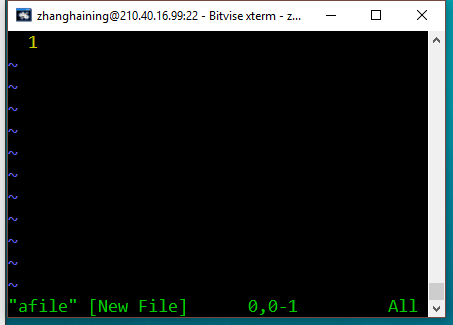
\includegraphics[width=1\linewidth]{BasicOperation/BOvim1}
\caption{vim open a file}
\label{BOvim1}
\end{figure}
在Figure \ref{BOvim1}中:最左侧的$\sim$代表当前行是空行,最下面是状态栏(显示了文件名,当前光标所在位置等信息)。vim的这种状态称为一般模式。

\subsubsection{插入文本}
在一般模式下,可以按iIoOaA这几个字符中的一个进行插入字符或行的操作。如果按下了i,则进入了插入状态,如Figure \ref{BOvim2}所示。
\begin{figure}
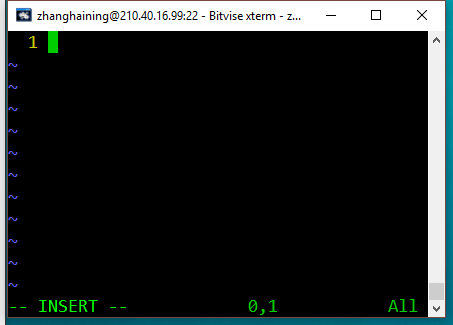
\includegraphics[width=1\linewidth]{BasicOperation/BOvim2}
\caption{insert in vim}
\label{BOvim2}
\end{figure}
可以看到Figure \ref{BOvim2}中左下状态栏中有insert字样,此时可以进行文件输入,直到按下esc键,按下esc键后,vim又会重返一般模式。
\subsubsection{删除文本和移动光标}
在一般模式下,可以按下hjkl这4个键其中之一进行光标的移动(一次移动一个字符或一行),也可以按下w键将光标移动到下一个单词的词首,或b键移动到上一个单词的词首。

如要删除某个字符可将光标移动到该字符上,然后按x键,如要删除一行,则将光标移动到那一行,然后按dd(d键连按两次)。
\subsubsection{保存文件和退出vim}
在一般模式下,按下:键,输入w即可完成文件的保存,输入q键即可退出vim,输入wq则可以完成保存并退出。
如Figure \ref{BOvim3}所示。
\begin{figure}
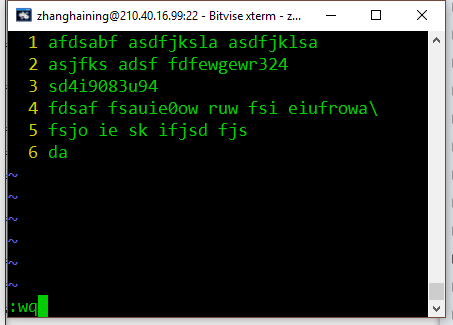
\includegraphics[width=1\linewidth]{BasicOperation/BOvim3}
\caption{save and quit}
\label{BOvim3}
\end{figure}
\subsection{重定向和管道}
重定向就是将数据流的目的地进行改变的一种机制。
\begin{verbatim}
$ cat afile > bfile
$ cat afile >> bfile
$ find / -name "shadow" 2> findErr
/usr/share/texlive/texmf-dist/tex/latex/shadow
/usr/share/texlive/texmf-dist/doc/latex/shadow
/etc/shadow
$ find / -name "shadow" > findLOG 2>&1
$ wc -l afile bfile findErr findLOG
6 afile
12 bfile
2969 findErr
2981 findLOG
5968 total
\end{verbatim}
管道是将数据流在程序(命令)间进行传递的一种机制,即将一个命令的输出做为另一个命令的输入。
\begin{verbatim}
$ cat findErr | head -5
find: ‘/lost+found’: Permission denied
find: ‘/mnt/public/lost+found’: Permission denied
find: ‘/mnt/share/temp’: Permission denied
find: ‘/run/sudo’: Permission denied
find: ‘/run/svnserve’: Permission denied
$ cat findErr | head -5| tail -2
find: ‘/run/sudo’: Permission denied
find: ‘/run/svnserve’: Permission denied
$ cat findLOG | grep -v "denied"
/usr/src/kernels/4.1.13-100.fc21.x86_64/include/config/kasan/shadow
/usr/src/debug/glibc-2.20/shadow
/usr/share/texlive/texmf-dist/tex/latex/shadow
/usr/share/texlive/texmf-dist/doc/latex/shadow
/etc/shadow
$ cat findLOG | grep "denied"|head -2
find: ‘/lost+found’: Permission denied
find: ‘/mnt/public/lost+found’: Permission denied
\end{verbatim}
